\chapter{Lecture 25 - Heat and Wave Equation with MATLAB}
\label{ch:lec25}
\section{Objectives}
\begin{itemize}
\item Describe the details of how to use MATLAB to construct approximate solutions to the heat and wave equations.
\item Illustrate how to create an animation with MATLAB; and
\item show an effective method for creating 2D plots with MATLAB.
\end{itemize}
\setcounter{lstannotation}{0} %hack to try and re-set annotation counter.

\section{Introduction}
In the past two lectures we have invested considerable time in the solution of two boundary value problems using the method of separation of variables.  When I teach this course I find that, during those lectures, there is little time available to spend going into the details of the MATLAB code created, essentially, to visualize the solution. Nonetheless it is often the case that a large fraction of the students have only modest proficiency in using MATLAB.\marginnote{Proficiency levels vary but students have had as much as two years under their belt using MATLAB to as little as two or three weeks.}  In this lecture we focus on the MATLAB details.  The hope is that students will come away with at least an introduction to the bare-minimum of MATLAB tools that will allow them to complete homework assignments.

\section{Example Heat Equation}

\marginnote[-1.0cm]{Take a moment to consider the units used in this boundary value problem.  If you believe the units provided for density, thermal conductivity, and specific heat, simple ``unit arithmetic'' shows that the thermal diffusivity should have units of cm\textsuperscript{2}/s.  What are the units of $\sfrac{\partial^2 u }{\partial x^2}$? Answer: $\sfrac{^{\circ}\text{C}}{\text{cm}^2}$.  What are the units of $\sfrac{\partial u}{\partial t}$?  Answer: $\sfrac{^{\circ}\text{C}}{\text{s}}$.  From this it should be clear that, indeed, the units are the same on the left and right side of the governing equation---as it \emph{must} be in order to be correct.  My point is that it does not take a tremendous amount of mathematical skill to check these things but you should \emph{always} check them.  If you do so, then you will definitely increase your confidence that you know what is going on; you may also save yourself from an embarrassing error.}
\noindent\textbf{Problem Statement: } Find the temperature $u(x,t)$ of a bar of silver of length 10cm.  The density is 10.6 g/cm\textsuperscript{3}, thermal conductivity is 1.04 cal/cm-s-$^{\circ}$C, and the specific heat is 0.056 cal/g-$^{\circ}$C.  The bar is perfectly insulated laterally with ends kept at 0$^{\circ}$C.  The initial temperature, $f(x)$, is given by: $f(x)=4-0.8\left|x-5\right|^{\circ}$C.  From this physical description of the problem, we formulate the following boundary value problem:
\begin{table}[h]
\begin{tabular}{l l}
$\substack{\text{Governing} \\\text{Equation}}: $& $\frac{\partial u}{\partial t} = \alpha^2 \frac{\partial^2 u}{\partial x^2}, \ \ \alpha>0, \ \ 0<x<10, \ \ t>0$ \\
& \\
$\substack{\text{Boundary} \\ \text{Conditions}}: $& $u(0,t)=0, \ \ u(10,t) = 0, \ \ t>0$\\
& \\
$\substack{\text{Initial} \\ \text{Conditions}}: $ & $u(x,0) = f(x) = 4-0.8\left|x-5\right|, \ \ 0<x<10 $ \\
\end{tabular}
\end{table} 

\vspace{4.0cm}

\marginnote[-3.0cm]{Being able to translate this kind of a description of a problem into a properly formulated boundary value problem that you can solve is a key skill you should develop from this course.}



\noindent\textbf{Analytic Solution: } 
\begin{equation}
u(x,t) = \sum\limits_{n=1}^{\infty} c_n \sin{\frac{n \pi x}{10}}e^{-\left(\frac{\alpha n \pi}{10}\right)^2t}
\label{eq:lec25-ex1-sol}
\end{equation}
where $\alpha^2 = \frac{k}{\rho c_p} = \frac{1.04}{(10.6)(0.056)} \text{cm\textsuperscript{2}}/\text{s}$ and the coefficients $c_n$ are given by:
\begin{equation*}
c_n = \frac{2}{10}\int_{0}^{10} \left(4-0.8\left|x-5\right| \right)\sin{\frac{n \pi x}{10}} \ dx
\end{equation*}

\vspace{0.5cm}

\noindent\textbf{MATLAB tasks:}
\begin{enumerate}
\item Construct an approximate representation of the solution in MATLAB including $N=50$ terms of the infinite series.
\item Create a plot of the solution at t = 0, 1, and 10 seconds.
\item Create an animation of the time-dependent temperature profile that you can save and incorporate, for example, in a presentation.
\item Visualize the time-dependent temperature profile using a 2D surface plot.
\end{enumerate}

We will tackle these tasks one at a time.

\vspace{0.25cm}

\noindent\textbf{Task \#1: } Construct an approximate representation of the solution in MATLAB including $N=50$ terms of the infinite series.  

\vspace{0.25cm} 

\noindent In this section of the code we clean out the workspace and provide basic given input data.
\marginnote{ 

\vspace{0.2cm}

\ref{lst:ann25-1-1} It is a good idea to include units and a brief statement indicating what a variable represents.  It may be easy to remember that, for instance, \lstinline[style=myMatlab]{L=10, \% cm} refers to the length but it is less easy to remember that \lstinline[style=myMatlab]{alpha_sq} refers to the thermal diffusivity.

\vspace{0.2cm}

\ref{lst:ann25-1-2} Make sure you fully understand how these anonymous functions work.  The snippet: \lstinline[style=myMatlab]{F = @(x,n) ...} should be read: ``F is a function of x and n...''  The ``L'' that appears on the right hand sides is the same ``L'' defined as a parameter.  The fact that this works is one of the benefits of using anonymous functions.  Remember to write these anonymous functions so that they can accept vector inputs for $x$ and $n$.  Built-in functions like \lstinline[style=myMatlab]{integral()} will fail if the function you supply to be integrated \emph{cannot} accept vector inputs.

}
\begin{lstlisting}[name=lec25-ex1, style=myMatlab]
clear
clc
close 'all'

%% Heat Equation BVP & Solution
L = 10; % cm
alpha_sq = 1.752; % cm^2/s, thermal diffusivity of silver. /*!\annotation{lst:ann25-1-1}!*/

N = 50;

F = @(x,n) sin(n.*pi.*x./L); /*!\annotation{lst:ann25-1-2}!*/
G = @(t,n) exp(-((n.*pi./L).^2)*alpha_sq.*t);

f = @(x) 4 - 0.8*abs(x - 5);

\end{lstlisting}

\vspace{0.25cm}

\noindent Next we will initialize and build---term by term---a truncated version of the infinite series.
\marginnote{

\vspace{0.1cm}

\ref{lst:ann25-1-3} On the surface, this does not do much: it simply creates a variable \lstinline{u} that is a handle to a function of two variables and sets it's initial value to zero.  If we did not have this, however, we would have to create a special case in the \lstinline{for...end} loop to create it on the first trip through.


}
\begin{lstlisting}[name=lec25-ex1, style=myMatlab]
u = @(x,t) 0;/*!\annotation{lst:ann25-1-3}!*/
for n = 1:N
    % essentially doing the sine-series half-wave expansion
    % compute the coefficient
    cn = (2/L)*integral(@(x) f(x).*F(x,n),0,L);
    
    % add the term to the series solution
    u = @(x,t) u(x,t) + cn*F(x,n).*G(t,n);
end
\end{lstlisting}
At this point, our first task is done. The variable \lstinline{u} represents the truncated series solution and we can evaluate the function at any point $x$ or $t$ to get the solution.\sidenote[][-0.75cm]{Sadly, there isn't anything you can do to prevent a user from evaluating the function at invalid/inappropriate vales of $x$ or $t$.  For example, \lstinline{u(1994, -25)} is perfectly legal MATLAB code.}

\vspace{0.25cm}

\noindent\textbf{Task \#2: } Create a plot of the solution at t=0, 1, and 10 seconds. 

\setcounter{lstannotation}{0} %hack to try and re-set annotation counter.
\vspace{0.1cm}

\noindent Code to complete this is presented in the listing below.
\marginnote{

\vspace{0.15cm} 

\ref{lst:ann25-1-4} The \lstinline{\%\%} separates MATLAB code into sections that can be executed independently.  Breaking scripts into sections like this can simplify debugging and helps improve code readability.

\vspace{0.2cm} 

\ref{lst:ann25-1-5} Familiarize yourself with these ``LineSpec'' strings.  For plots with multiple data series you should try to make it easy to tell the difference between different data series even if the plot is viewed in black and white.

\vspace{0.05cm}

\ref{lst:ann25-1-6} Using the \lstinline[style=myMatlab]{'MarkerIndices'} argument allows you to specify which data indices get annotated with a marker (when the line specification includes a marker).  The value \lstinline[style=myMatlab]{1:50:Nx} in this case results in 1 out of every 50 data points having a marker applied.  Experiment with this and see what the plot looks like if you omit this name-value pair.

}
\begin{lstlisting}[name=lec25-ex1, style=myMatlab]
%% Plot the result for fixed times /*!\annotation{lst:ann25-1-4}!*/
% make a discrete X-axis
Nx = 1000;
X = linspace(0,L,Nx);
figure(1)
plot(X,u(X,0),'-ob',...
    X,u(X,1),'-.g',... /*!\annotation{lst:ann25-1-5}!*/
    X,u(X,10),'--r','MarkerIndices',1:50:Nx,'linewidth',3); /*!\annotation{lst:ann25-1-6}!*/
title('Lecture #25 Example','fontsize',16,'fontweight','bold');
xlabel('X [cm]','fontsize',14,'fontweight','bold');
ylabel('u(X,t)   [^{\circ}C]',... /*!\annotation{lst:ann25-1-7}!*/
    'fontsize',14,'fontweight','bold');
grid on
set(gca,'fontsize',12,'fontweight','bold');
legend('t = 0','t = 1','t = 10'); /*!\annotation{lst:ann25-1-8}!*/
\end{lstlisting}

\vspace{0.15cm}

\noindent \ref{lst:ann25-1-7} The string snippet `\string^\{\string\circ \} C' is \LaTeX mark-up and is rendered by MATLAB as $^{\circ}$C.  While not strictly necessary, use of such mark-up can make a plot more attractive.

\vspace{0.15cm}

\noindent \ref{lst:ann25-1-8} Obviously use of a legend makes a plot easier to read.  MATLAB also includes an optional argument named \lstinline{'location'} that can be used with values such as: \lstinline{'northwest','southwest','northeast','southeast','best'}...etc---that allow you to place a legend such that it does not interfere with reading the plot.  Consult the MATLAB documentation for more information about legends.

\vspace{0.15cm}

\noindent A plot created by the code snippet above is shown in Figure \ref{fig:lec25-ex1-plt1}.
\begin{marginfigure}
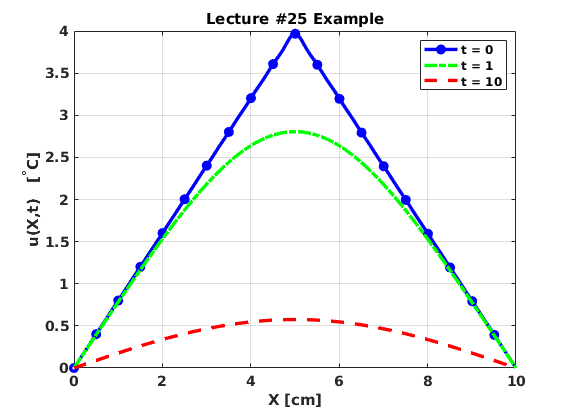
\includegraphics{lec25-ex1-plt1.png}
\caption{Plot of heat equation example at t=0,1, and 10 seconds}
\label{fig:lec25-ex1-plt1}
\end{marginfigure}

\vspace{0.25cm}

\setcounter{lstannotation}{0} %hack to try and re-set annotation counter.
\noindent\textbf{Task \#3: } Create an animation of the time-dependent temperature profile that you can save and incorporate, for example, in a presentation.

\vspace{0.15cm}

\noindent For this task we will first create a simple time-dependent plot that you might use for a homework assignment, independent research project, or for your capstone.  The goal is to gain understanding of the transient behavior of this physical system.

\marginnote{
\vspace{0.25cm}

\ref{lst:ann25-1-9} Discretize time as desired.  

\vspace{0.15cm} 

\ref{lst:ann25-1-10} The \lstinline[style=myMatlab]{sprintf()} allows you to create formatted strings for the title.  In this case, we include the time, in seconds.  The snippet \lstinline[style=myMatlab]{'\%5.3g'} is a formatting string; in this case the value returned from \lstinline[style=MyMatlab]{T(n)} is placed here in a field 5 digits wide with up to 3 digits to the right of the decimal point.  The character `g' tells MATLAB to render the number either in fixed-point notation (e.g. 3.14) or scientific notation (e.g. 1.6e9) whichever is more compact.

\vspace{0.15cm}

\ref{lst:ann25-1-11} This sets the axis limits \lstinline[style=myMatlab]{axis([xmin xmax ymin ymax])}.  The default behavior is to re-scale the plot to fit the max/min plotted values.  For transient simulations this can make changes to the temperature profile harder to understand.  Try running this script without this command to better understand the effect.

}
\begin{lstlisting}[name=lec25-ex1, style=myMatlab]
%% Simple time-dependent plot 
Tmax = 15; % s
NT = 30;
T = linspace(0,Tmax,NT); /*!\annotation{lst:ann25-1-9}!*/
figure(2)
for n = 1:NT
   plot(X,u(X,T(n)),'-b','linewidth',2)
   title_str = sprintf('Lecture #25 Example, t = %5.3g',T(n)); /*!\annotation{lst:ann25-1-10}!*/
   title(title_str,'fontsize',16,'fontweight','bold');
   xlabel('X','fontsize',14,'fontweight','bold');
   ylabel('u(X,T)','fontsize',14,'fontweight','bold');
   grid on
   set(gca,'fontsize',12,'fontweight','bold');
   axis([0 L -0.2 4.5]); /*!\annotation{lst:ann25-1-11}!*/
   pause(Tmax/(NT-1)); /*!\annotation{lst:ann25-1-12}!*/
end
\end{lstlisting}

\vspace{0.15cm}

\ref{lst:ann25-1-12} This command causes MATLAB to pause slightly before starting the next iteration in the for-loop.  The argument to the \lstinline[style=myMatlab]{pause()} function is the duration (in seconds) of the pause.  For some systems this pause also allows the graphics system a chance to update between iterations in the for-loop.  (i.e. if you omit the pause, you may not see your plot update until the very end and miss all of the transient behavior.)

\newthought{This plot is good} for routine homework or analysis that you do not intend to present publicly. Sometimes you \emph{do} want to show a time-dependent plot of a system you are analyzing but you do not want to run the MATLAB script that created the plot during the presentation.  A good option is to create a movie that can be played from most computers and/or can be embedded in a presentation.  The next code block accomplishes this task.
\marginnote{

\vspace{0.3cm}

\ref{lst:ann25-1-13} This creates an array of structures; each structure has two fields, one for the color-data \lstinline{'cdata'}, and one for the color-map \lstinline{'colormap'}. A structure is a data-type that we use infrequently for this course. If you wanted, for instance, to access the 3\textsuperscript{rd} frame color-data you would use the command:

\vspace{0.1cm}

 \lstinline{FRAMES(3).cdata} 

\vspace{1.5cm}

\ref{lst:ann25-1-14} the command \lstinline{gcf} means ``get current frame.''  In this line, the n\textsuperscript{th} frame of the animation is saved to the n\textsuperscript{th} FRAMES structure.

}
\begin{lstlisting}[style=myMatlab, name=lec25-ex1]
%% Save the time-dependent plot as a Movie 
FRAMES(NT) = struct('cdata',[],'colormap',[]); /*!\annotation{lst:ann25-1-13}!*/
figure(3)
for n = 1:NT
    plot(X,u(X,T(n)),'-b','linewidth',3);
    title_str = ...
        sprintf('Lecture #25 Example, t = %g ',T(n));
    title(title_str,'fontsize',16,'fontweight','bold');
    xlabel('X','fontsize',14,'fontweight','bold');
    ylabel('u(X,T)','fontsize',14,'fontweight','bold');
    grid on
    set(gca,'fontsize',12,'fontweight','bold');
    axis([0 L -0.2 4.5]);
    drawnow % ensures graphics pipeline is complete/"flushed"
    FRAMES(n) = getframe(gcf); /*!\annotation{lst:ann25-1-14}!*/
end

%% play the movie
fig = figure(4);
movie(fig,FRAMES,10); % last argument is frames-per-second

%% Write frames to AVI file 
v = VideoWriter('TransientHeat.avi'); /*!\annotation{lst:ann25-1-15}!*/
open(v);
for n = 1:NT
   writeVideo(v,FRAMES(n)); 
end
close(v); /*!\annotation{lst:ann25-1-16}!*/
\end{lstlisting}
\marginnote[-2.5cm]{

\ref{lst:ann25-1-15} This function creates and opens an AVI file to which the \lstinline[style=myMatlab]{writeVideo()} function can write a video frame-by-frame. See MATLAB documentation for other supported video file types.

\vspace{0.15cm}

\ref{lst:ann25-1-16} Be a good citizen and close any files you open for writing. 

}


\vspace{0.25cm}
\setcounter{lstannotation}{0} %hack to try and re-set annotation counter.
\noindent\textbf{Task \#4: } Visualize the time-dependent temperature profile using a 2D surface plot.

\vspace{0.15cm}

\noindent Animations are nice but sometimes the splashy graphics is not needed and you just want to see how the temperature across the domain changes over time in a static image.  A surface plot is an excellent way to do this; the MATLAB built-in function that does the job is cunningly named \lstinline[style=myMatlab]{surf()} and is shown in the listing below.
\marginnote{

\vspace{0.3cm} 

\ref{lst:ann25-1-17} The \lstinline[style=myMatlab]{meshgrid()} function outputs 2D grid coordinates corresponding to the vector inputs for each dimension.  The output arrays \lstinline{XX} and \lstinline{TT} are suitable for use in the \lstinline[style=myMatlab]{surf()} function.

\vspace{0.2cm}



}
\begin{lstlisting}[style=myMatlab, name=lec25-ex1]
%% Plot the temperature vs time in a 2D plot using the surf function
[XX,TT] = meshgrid(X,T); /*!\annotation{lst:ann25-1-17}!*/
figure(5)
surf(XX,TT,u(XX,TT),'edgecolor','none'); /*!\annotation{lst:ann25-1-18}!*/
title('Lecture 25 Suface Plot Example',...
    'fontsize',18,'fontweight','bold');
xlabel('X [cm]','fontsize',16,'fontweight','bold');
ylabel('T [s]','fontsize',16,'fontweight','bold');
zlabel('u(X,T)  [^{\circ}C]','fontsize',16,...
    'fontweight','bold');
\end{lstlisting}

\vspace{0.2cm}

\ref{lst:ann25-1-18} The \lstinline[style=myMatlab]{surf(XX,YY,ZZ)} function takes at least three arguments; in this case the first two are used by the output of \lstinline[style=myMatlab]{meshgrid()} and the last is created by supplying the \lstinline{XX} and \lstinline{TT} arrays to our approximate solution---\lstinline{u(x,y)}---which serves as the height (or z-coordinate) of the surface plot at each point. The name-value pair: \lstinline{'edgecolor','none'} suppresses the (by default) black grid line that delineate the mesh created with \lstinline{XX} and \lstinline{TT}.  For high-resolution meshes the grid lines would obscure the color-map used to highlight the solution. (Try omitting this name-value pair and observe the effect.)

\vspace{0.2cm}

\noindent The resulting surface plot is shown in Figure \ref{fig:lec25-ex1-surf-plt}.

\begin{marginfigure}
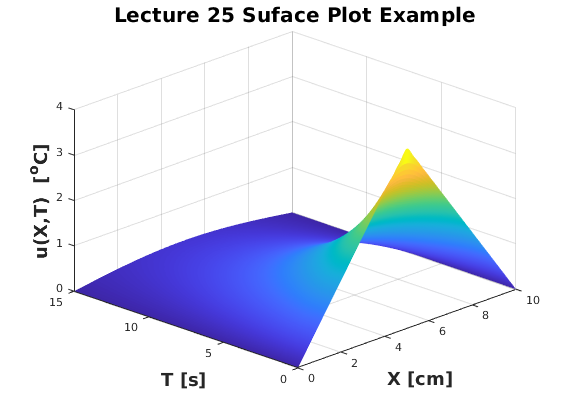
\includegraphics{lec25-ex1-surf-plt.png}
\caption{Surface plot of heat equation example.}
\label{fig:lec25-ex1-surf-plt}
\end{marginfigure}

\section{Example Wave Equation}

For this we will consider the wave equation example analyzed in Lecture 24.  The code may be familiar by this point, but since we did not take the time to go through the MATLAB implementation in detail before, we will take the time here.

\vspace{3.0cm}

\noindent The boundary value problem is given as:
\begin{table}
\begin{tabular}{l l}
$\substack{\text{Governing} \\\text{Equation}}: $& $\frac{\partial^2 u}{\partial t^2} = \alpha^2 \frac{\partial^2 u}{\partial x^2}, \ \ \alpha > 0, \ a<x<b$  \\
& \\
$\substack{\text{Boundary} \\ \text{Conditions}}: $& $u(0,t)=0, \ \ u(L,t) = 0, \ \ t>0$\\
& \\
$\substack{\text{Initial} \\ \text{Conditions}}: $ & $u(x,0) = f(x), \ \ u_{t}(x,0) = g(x), \ \ 0<x<L $ \\
\end{tabular}
\end{table}
where the length is given by $L=3$, wave speed is 1, and the initial conditions are given by:
\begin{align*}
f(x) &= \begin{cases} \frac{2}{3x}, & 0 < x < \frac{3}{2} \\ \frac{2}{3}(3-x), & \frac{3}{2} \le x < 3 \end{cases} \\
g(x) &= 0
\end{align*}

\vspace{0.25cm}
\noindent The analytic solution is:
\begin{align*}
u(x,t) &= \sum\limits_{n=1}^{\infty} \left(a_n \cos{\alpha \frac{n \pi t}{L}} + b_n \sin{\alpha \frac{n \pi t}{L}} \right) \sin{\alpha \frac{n \pi x}{L}} \\
a_n &= \frac{2}{L} \int_{0}^{L} f(x) \sin{\alpha_n \frac{n \pi x}{L}} \ dx \\
b_n &= \frac{2}{\alpha n \pi} \int_{0}^{L} g(x) \sin{\alpha \frac{n \pi x}{L}} \ dx
\end{align*}

\setcounter{lstannotation}{0} %hack to try and re-set annotation counter.

\vspace{0.2cm}

\noindent We begin, again, by cleaning out the workspace and command window and closing all figure windows; then we declare basic problem parameters.
\marginnote{

\vspace{0.5cm}

\ref{lst:ann25-2-1} Recall that $\alpha^2 = \sfrac{T}{\rho}$ where $T$ is the tension (force) and $\rho$ is the density.  Unit analysis shows that $\alpha^2$ has units of: $\sfrac{m \sfrac{L}{t^2}}{\sfrac{m}{L^3}} = \sfrac{L^2}{s^2}$ where $m$ is mass, $L$ is length, and $t$ is time.  Thus $\alpha$ has units of $\sfrac{L}{s}$ and we call it the ``wave speed''.  Now is also a good time to examine the governing equation of the boundary value problem and confirm to yourself that the units make sense.

\vspace{0.2cm}

\ref{lst:ann25-2-2} Notice that the \lstinline{L} from the parameter list is used for the second argument of \lstinline[style=myMatlab]{ex1(x,L)}.  

}
\begin{lstlisting}[name=lec25-ex2, style=myMatlab]
clear
clc
close 'all'

%% Example Problem
L = 3;
alpha_sq = 1;% T/rho
alpha = sqrt(alpha_sq); /*!\annotation{lst:ann25-2-1}!*/
N = 50;

f = @(x) ex1(x,L);/*!\annotation{lst:ann25-2-2}!*/
g = @(x) x.*0; /*!\annotation{lst:ann25-2-3}!*/
\end{lstlisting}
\vspace{0.2cm}

\ref{lst:ann25-2-3} At first glance it would appear to be easier to simply make the assignment: \lstinline[style=myMatlab]{g = 0;}.  We do it this way so that the follow-on code can be written in a way that assumes that \lstinline{g} is a function of $x$---i.e. the code \lstinline[style=myMatlab]{integral(@(x) g(x).*sin(n*pi*x./L,0,L)} does not result in an error. In the future, if we replace $g(x)=0$ with a  non-trivial function of $x$, for example, $g(x)=\sin{x}$ everything will work as expected.

\vspace{3.5cm}

\noindent Next we will initialize our approximate solution and built it up term-by-term.

\begin{lstlisting}[style=myMatlab, name=lec25-ex2]
u = @(x,t) 0;
for n = 1:N
    % compute the coefficients
    an = (2/L)*integral(@(x) f(x).*sin(n*pi*x./L),0,L);
    bn = ...
        (2/(alpha*n*pi))*...
        integral(@(x) g(x).*sin(n*pi*x./L),0,L);
    % update the approximate solution
    u = @(x,t) u(x,t) + ...
        (an*cos(alpha.*n*pi*t./L) + ...
        bn*sin(alpha.*n*pi*t./L)).*sin(n*pi*x./L); 
end
\end{lstlisting}
\marginnote[-3.5cm]{ This equation has two expansion coefficients: $a_n$ and $b_n$, unlike the heat equation which had only one but incorporation of that added complexity in MATLAB is straightforward.
}

\vspace{0.25cm}

\noindent Now that the approximate solution has been computed, we can plot the results.  We may, if we wish, create a dynamic plot much like we did with the heat equation so that we can see the wave behavior in action.

\begin{lstlisting}[style=myMatlab, name=lec25-ex2]
%% make discrete space and time space vectors
Tmax = 3;
NT = 50;
T = linspace(0,Tmax,NT);
Nx = 500;
X = linspace(0,L,Nx);

%% create time-dependent plot
figure(1)
for n = 1:NT
   plot(X,u(X,T(n)),'-b','linewidth',3); 
   title_str = sprintf('Lecture 24 Example, t = %g ',T(n));
   title(title_str,'fontsize',16,'fontweight','bold');
   xlabel('X','fontsize',14,'fontweight','bold');
   ylabel('u(X,T)','fontsize',14,'fontweight','bold');
   grid on
   set(gca,'fontsize',12,'fontweight','bold');
   axis([0 L -1.5 1.5]);
   pause(Tmax/(NT-1));
end
\end{lstlisting}

\vspace{0.25cm}

\noindent Or we can make a single plot with multiple data-series as shown in Figure \ref{fig:lec25-ex2-plt1}:
\begin{marginfigure}
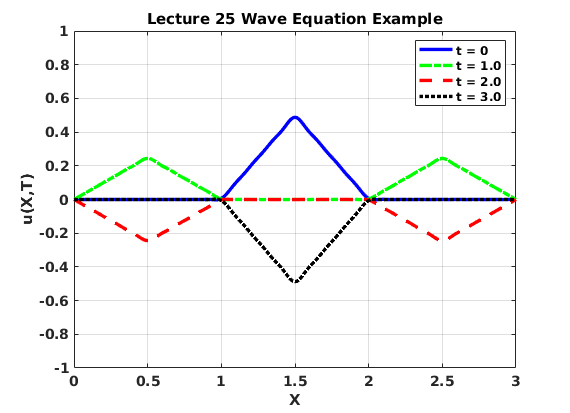
\includegraphics{lec25-ex2-plt1.png}
\caption{Plot of wave equation example problem at t=0, 1.0, 2.0, and 3.0 sec.}
\label{fig:lec25-ex2-plt1}
\end{marginfigure}

\begin{lstlisting}[style=myMatlab, name=lec25-ex2]
%% fixed plot, multiple data series
figure(2)
plot(X,u(X,0),'-b',...
    X,u(X,1.0),'-.g',...
    X,u(X,2.0),'--r',...
    X,u(X,3.0),':k','linewidth',3);
title('Lecture 25 Wave Equation Example',...
    'fontsize',16,'fontweight','bold');
xlabel('X','fontsize',14,'fontweight','bold');
ylabel('u(X,T)','fontsize',14,...
    'fontweight','bold');
grid on
set(gca,'fontsize',12,'fontweight','bold');
axis([0 L -1.0 1.0]);
legend('t = 0','t = 1.0','t = 2.0','t = 3.0',...
    'location','best');
\end{lstlisting}

\vspace{1.0cm}

\noindent Lest we forget, we also need to define the function \lstinline[style=myMatlab]{ex1(x,L)}.  We choose to do this as a \emph{local function} which means that it has to be placed \emph{at the end} of the script file.

\begin{lstlisting}[style=myMatlab, name=lec25-ex2]
%% Local functions
function y = ex1(x,L)
[m,n] = size(x);
y = nan(m,n);
for i = 1:length(x)
   if (x(i)>0)&& (x(i) < L/2)
       y(i) = (2/3).*x(i);
   elseif(x(i) >= L/2) && (x(i)<L)
       y(i) = (2/3)*(L - x(i));
   end
end
end
\end{lstlisting}
